\documentclass[12pt,a4paper]{article}
\usepackage[UTF8]{ctex}     %先引入ctex
\usepackage[utf8]{inputenc} %再引入inputenc
\usepackage{graphicx}
% \usepackage{lazylatex}
\usepackage{minted}
\usepackage{amsmath}
\usepackage{bookmark}
\usepackage{enumerate}
\usepackage{geometry}
\usepackage{array}
% \tcbuselibrary{documentation}
\graphicspath{{img/}}
% 边距
\geometry{left=2.0cm,right=2.0cm,top=2.0cm,bottom=3.0cm}
% 大题
\newenvironment{problems}{\begin{list}{}{\renewcommand{\makelabel}[1]{\textbf{##1}.\hfil}}}{\end{list}}
% 小题
\newenvironment{steps}{\begin{list}{}{\renewcommand{\makelabel}[1]{(##1)\hfil}}}{\end{list}}
% 答
\providecommand{\ans}{\textbf{答}:~}
% 解
\providecommand{\sol}{\textbf{解}.~}

\setminted{breaklines,autogobble,frame=lines,framesep=2mm,fontsize=\scriptsize}

\begin{document}
\title{\normalsize \underline{计算机系统结构(A)}\\\LARGE 第 2 次作业}
\author{李子龙 518070910095}
\date{\today}
\maketitle

\begin{problems}
    \item[1.] \textbf{单周期处理器控制逻辑}
    
    % 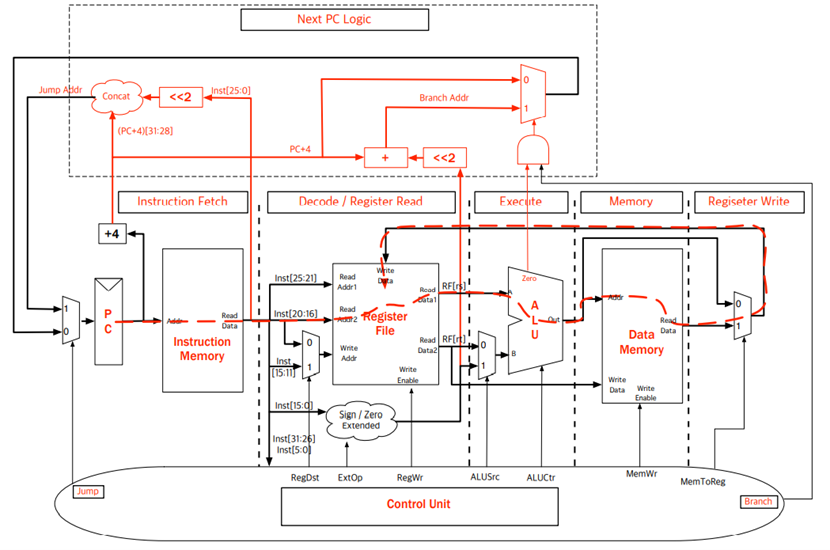
\includegraphics[width=0.8\textwidth]{p1.png}

    % 这个表格给出了算术逻辑单元每个操作的ALUCtr值:

    % \begin{tabular}{|c|cccccc|}
    %     \hline
    %     Operation & AND & OR & ADD & SUB & SLT & XOR \\
    %     \hline
    %     ALUStr & 0000 & 0001 & 0010 & 0110 & 0111 & 1100\\
    %     \hline
    % \end{tabular}

    在下表中填写出上图中各个控制信号的数值:
    
    \begin{tabular}{c|ccccccc}
        & \multicolumn{7}{c}{Control Signals}\\
        Instrs. & \sffamily RegDst &\sffamily ExtOp &\sffamily ALUSrc &\sffamily ALUCtr &\sffamily MemWr &\sffamily MemtoReg &\sffamily RegWr \\ 
        \hline
        \ttfamily add & & & & & & & \\ 
        \ttfamily ori & & & & & & & \\
        \ttfamily lw  & & & & & & & \\ 
        \ttfamily sw  & & & & & & & \\ 
        \ttfamily beq & & & & & & & \\
        \ttfamily j   & & & & & & & \\
        \hline
    \end{tabular}


    \item[2] \textbf{单周期处理器的性能分析}
    
    % 时钟分析方法: 
    % \begin{itemize}
    %     \item 每个状态元件的输入信号必须在时上升沿之前稳定下来。
    %     \item 关键路径(critical path):电路中状态元件之间最长的延迟路径。 
    %     \item $t_{clk} \geq t_{clk-to-q} + t_{CL} + t_{setup}$, 其中 $t_{CL}$ 是组合逻辑中的关键路径。
    %     \item 如果我们把寄存器放在关键路径上,我们可以通过减少寄存器之间的逻辑量来缩短周期。
    % \end{itemize}
    % 电路元件的延时如下所示:

    % \begin{tabular}{c|m{4em}m{4em}m{3em}m{3em}m{4em}m{4em}m{4em}m{4em}}
    %     Element & Register clk-to-q & Register Setup & MUX & ALU & Mem Read & Mem Write & RegFile Read & RegFile Setup\\
    %     Paramenter & $t_{clk-to-q}$ & $t_{setup}$ & $t_{mux}$ & $t_{ALU}$ & $t_{MEMread}$ & $t_{MEMwrite}$ & $t_{RFread}$ & $T_{RFsetup}$\\
    %     \hline
    %     Delay & 30 & 20 & 25 & 200 & 250 & 200 & 150 & 20 \\
    %     \hline
    % \end{tabular}
 
    % 关于硬件中的时钟的一些术语说明:
    % \begin{itemize}
    %     \item 时钟(CLK):使系统同步的稳定方波
    %     \item 启动时间(setup time):在时钟边沿之前,输入必须稳定的时间
    %     \item 保持时间(hold time):在时钟边沿之后,输入必须稳定的时间
    %     \item “CLK-to-Q”延迟(“CLK-to-Q” delay):从时钟边沿测量,改变输出需要多长时间
    %     \item 周期(period)=最大延迟=“CLK-to-Q”延迟+CL延迟+启动时间
    %     \item 时钟频率=1/周期(即周期的倒数)
    % \end{itemize}

    回答问题:
    \begin{enumerate}
        \item 用到关键路径(critical path)的指令是哪一条?
        \item 最小时钟周期 $t_{clk}$是多少?最大时钟频率$f_{clk}$是什么?假设$t_{clk-to-q}>$ 保持时间(hold time). 
    \end{enumerate}

    \item[3] \textbf{流水线处理器设计(Pipelined CPU Design)} 
    % 现在,我们将使用流水线方法来优化一个单周期处理器。流水线虽然增加了单个任务的延迟,但它可以减少时钟周期,提高吞吐量。 在流水线处理器中,多条指令重叠执行,体现了指令级并行性。
    % 为了设计流水线,我们已经将单周期处理器分成五个阶段,在每两个阶段之间增加流水段寄存器。
    % 接下来进行性能分析:

    % 我们将使用与上一题相同的时钟参数:

    % \begin{tabular}{c|m{4em}m{4em}m{3em}m{3em}m{4em}m{4em}m{4em}m{4em}}
    %     Element & Register clk-to-q & Register Setup & MUX & ALU & Mem Read & Mem Write & RegFile Read & RegFile Setup\\
    %     Paramenter & $t_{clk-to-q}$ & $t_{setup}$ & $t_{mux}$ & $t_{ALU}$ & $t_{MEMread}$ & $t_{MEMwrite}$ & $t_{RFread}$ & $T_{RFsetup}$\\
    %     \hline
    %     Delay & 30 & 20 & 25 & 200 & 250 & 200 & 150 & 20 \\
    %     \hline
    % \end{tabular}

    回答问题:
    \begin{itemize}
        \item 这个五阶段流水线处理器的最小时钟周期长度和最大时钟频率分别是多少?
        \item 相比于单周期处理器,性能加速比(speed up)是多少?为什么加速比会小于5?
    \end{itemize}

    \item[4] \textbf{控制冒险(Control Hazard) }
    
    问题:
    考虑填充转移延迟槽,我们需要重新排列以下几组指令,如果实在找不到指令填充延迟槽,你可能需要插入一条nop指令。

    \begin{tabular}{>{\ttfamily}l>{\ttfamily}l|>{\ttfamily}l>{\ttfamily}l}
        \bfseries Set 1 &\bfseries Reordered set 1 &\bfseries Set 2 &\bfseries Reordered set 2\\
        \hline
        addiu \$t0,\$t1,5 & & addiu \$t0,\$t1,5 & \\
        ori \$t2,\$t3,0xff & & ori \$t2,\$t3,0xff & \\
        beq \$t0,\$s0,label & & beq \$t0,\$t2,label & \\
        lw \$t4,0(\$0) & & lw \$t4,0(\$0) & \\
    \end{tabular}

    \item[5] \textbf{转移延迟槽}
    
    如果需要第二种设计能达到第一种设计的性能,转移预测的准确度应该为多少?

    \item[6] \textbf{指令调度}

    假定在一个有转发(forwarding)功能的五段流水线中执行以下程序段,则可以怎样调整以下指令序列使其性能达到最好?
    \begin{minted}{asm}
lw   $2, 100($6)
add  $2, $2, $3
lw   $3, 200($7)
add  $6, $4, $7
sub  $3, $4, $6
lw   $2, 300($8)
beq  $2, $8, Loop
    \end{minted}

    \item[7] \textbf{中断}
 
当MIPS处理器在执行一条除法指令时,发生了除数为0异常(exception)。那么此时处理器就要进行中断处理。在中断处理过程中,最开始的一部分工作由硬件完成,描述一下: 
\begin{enumerate}
    \item 中断处理开始的阶段,硬件需要完成哪些工作,保存哪些状态? 
    \item 如果中断处理程序(interrupt handler)需要读寄存器R5, R6, R7, 写寄存器R5, R8, R10, 那么中断处理程序应该在一开始保留哪几个寄存器的值?
    \item ERET(中断返回)指令会触发硬件完成哪些动作?
    \item 如果一条指令在执行阶段,即发生了“指令地址错误“异常,又发生了”ALU运算溢出“异常,那么这条指令被中断时,原因寄存器(cause register)中记录的中断原因,应该是哪一个?
\end{enumerate}
    

\end{problems}
\end{document}